\documentclass[paper=a4, fontsize=11pt]{scrartcl} % A4 paper and 11pt font size
\usepackage[T1]{fontenc} % Use 8-bit encoding that has 256 glyphs
\usepackage[english]{babel} % English language/hyphenation
\usepackage{multirow}
\usepackage{graphicx}
\usepackage{amsmath,amsfonts,amsthm} % Math packages
\usepackage{sectsty} % Allows customizing section commands
\allsectionsfont{\centering \normalfont\scshape} % Make all sections centered, the default font and small caps

\usepackage{fancyhdr} % Custom headers and footers
\pagestyle{fancyplain} % Makes all pages in the document conform to the custom headers and footers
\fancyhead{} % No page header - if you want one, create it in the same way as the footers below
\fancyfoot[L]{} % Empty left footer
\fancyfoot[C]{} % Empty center footer
\fancyfoot[R]{\thepage} % Page numbering for right footer
\renewcommand{\headrulewidth}{0pt} % Remove header underlines
\renewcommand{\footrulewidth}{0pt} % Remove footer underlines
\setlength{\headheight}{13.6pt} % Customize the height of the header

\graphicspath{ {../Plots/} }

\newcommand{\horrule}[1]{\rule{\linewidth}{#1}} % Create horizontal rule command with 1 argument of height

\title{	
\normalfont \normalsize 
\textsc{TMA4220 Numerical Solution of Differential Equations by element methods} \\ [25pt] % Your university, school and/or department name(s)
\horrule{0.5pt} \\[0.4cm] % Thin top horizontal rule
\huge Part 1 \\ % The assignment title
\horrule{2pt} \\[0.5cm] % Thick bottom horizontal rule
}

\author{Candidate numbers} % Your name

\date{\normalsize\today} % Today's date or a custom date

\begin{document}
\maketitle

Introduction :D

\section{Gaussian quadrature}
Evaluation of definite integrals is an integral part of every finite element code. The integrals vary in complexity and many does not even have known analytical solutions. One general way find approximate solutions to them is by  \textit{Gaussian quadrature}
\[ \int_{\hat{\Omega}} \! g(\mathbf{\zeta}) \, \mathrm{d}\mathbf{\zeta} \approx \sum_{q=1}^{N_q} \rho_{q}g(\mathbf{\zeta}_q).
\]
The function $g(\mathbf{\zeta})$ is evaluated in the $N_q$ vector quadrature points, $\mathbf{\zeta}_q$, with $\rho_q$ as the associated Gaussian weights. In all numerical quadratures, the points and weights are given on a reference domain, $\hat{\Omega}$. It is therefore important to have a map from this domain to the domain at hand.

\subsection{1D quadrature}

In 1D $\hat{\Omega}=[-1,1]$. So for $\zeta \in [-1,1]$ the mapping
\[ x=\frac{1}{2} \left((b-a) \zeta +(b+a)\right)
\]

takes any point onto a general domain [a,b] and gives the approximation

\[ \int_{\Omega} \! g(x) \, \mathrm{d}x = \int_{\hat{\Omega}} \! g\left(x(\zeta)\right) \, \frac{\mathrm{d}x}{\mathrm{d}\zeta}\mathrm{d}\zeta \approx \frac{1}{2}(b-a) \sum_{q=1}^{N_q} \rho_{q}g(x(\zeta_q)).
\]

\subsection{2D quadrature}
In higher dimensions a bit more care is needed. Consider triangles on the (x,y)-plane with corner points $\mathbf{p_i}=(x_i,y_i), i=1,2,3$. Then define the area coordinates 
\[ \zeta_i = \frac{A_i}{A}, \; i=1,2,3,\]
as indicated in figure [FIGURE OF AREA COORDINATES]. Now area coordinates $\zeta_i \in [0,1]$ map to physical coordinates $\mathbf{x}$ via

\[ \mathbf{x} = \zeta_1\mathbf{p_1} +\zeta_2\mathbf{p_2} +\zeta_3\mathbf{p_3}.
\]

Let the reference element be the triangle with corners in (0,0), (0,1) and (1,0) on the $(\xi,\eta)$-plane. Then the lowest order mapping corresponding in each corner is
\[ \mathbf{x}= \mathbf{p_1}(1-\xi-\eta) +\mathbf{p_2}\xi +\mathbf{p_3}\eta = J_k\left[ \begin{array}{c} \xi\\ \eta\\ \end{array} \right] + \mathbf{p_1},
\]
where $J_k$ is the Jacobian matrix of the transformation. The Jacobian determinant is then

\begin{equation}
|J(\xi,\eta)| = \mathrm{det}(J_k) = \begin{vmatrix}
  x_2-x_1 & x_3-x_1 \\
  y_2-y_1 & y_3-y_1 \\
\end{vmatrix}.
  \label{eq:jacobian2d}
\end{equation}

Gaussian quadrature points, $\zeta_q$, and weights, $\rho_q$, in area coordinates are given as triplets. The quadrature rules also introduce a scaling with the element size (here area), $T_\Omega$. The approximation of the integral is thus
\[ \int_{\Omega} \! g(\mathbf{x}) \, \mathrm{d}x\mathrm{d}y = \int_{\hat{\Omega}} \! g(\mathbf{x}) \, |J(\xi,\eta)| \mathrm{d}\xi \mathrm{d}\eta \approx T_{\hat{\Omega}} |J(\xi,\eta)| \sum_{q=1}^{N_q} \rho_{q}g(\mathbf{x}(\zeta_q)).
\]
Note that taking $g$ to be constant over the element gives $T_{\Omega}=T_{\hat{\Omega}} |J(\xi,\eta)|$. For our reference element the area is $T_{\hat{\Omega}}=1/2$.

\subsection{3D quadrature}
The extention into 3 dimensions and for tetrahedral elements is straight forward. Let

\[ \mathbf{x} = \zeta_1\mathbf{p_1} +\zeta_2\mathbf{p_2} +\zeta_3\mathbf{p_3} + \zeta_4\mathbf{p_4} 
\]
for $\mathbf{p_i} =(x_i,y_i,z_i)$ and the reference tetrahedral defined by the corner points $(0,0,0)$,$(0,1,0)$,$(0,0,1)$ and $(1,0,0)$ in the $(\xi,\eta,\psi)$-coordinate system. Then the mapping is

\[ \mathbf{x}= J_k\left[ \begin{array}{c} \xi\\ \eta\\ \psi \end{array} \right] + \mathbf{p_1}.
\]

where the columns of $J_k$ are given by $\mathbf{p_i}-\mathbf{p_1}$ for $i\neq1$ as in the 2D case. The integral over the element can be approximated by

\[ \int_{\Omega} \! g(\mathbf{x}) \, \mathrm{d}x\mathrm{d}y\mathrm{d}z  \approx T_{\hat{\Omega}} |J(\xi,\eta,\psi)| \sum_{q=1}^{N_q} \rho_{q}g(\mathbf{x}(\zeta_q)),
\]

where $T_{\hat{\Omega}}=1/6$ is the volume of the reference element.

\section{Poisson equation in 2 dimensions}

Consider the two-dimensional Poisson problem

\begin{equation}
\begin{aligned}
\nabla^2u(x,y) 	&= -f(x,y) \\
u(x,y)|_{r=1} 	&= 0,
\end{aligned}
\label{eq:poisson2d}
\end{equation}
on the domain $\Omega = \{(x,y) : x^2+y^2\leq 1\}$, and with $f$ given in polar coordinates as
\[ f(r,\theta)= -8\pi \cos(2\pi r^2)+16\pi^2r^2\sin(2\pi^2 r^2).\]

\subsection{Analytical solution}
An analytical solution to problem (\ref{eq:poisson2d}) is 

\begin{equation}
u(x,y)=\sin\left(2\pi(x^2+y^2)\right)
\label{eq:poisson2danal}
\end{equation}
since by direct computation

\[\nabla^2u(x,y) = \left( \frac{\partial^2}{\partial x^2} + \frac{\partial^2}{\partial y^2} \right) u(x,y) = \frac{\partial}{\partial x} 4\pi x\cos\left(2\pi(x^2+y^2)\right) + \frac{\partial}{\partial y} 4\pi y\cos\left(2\pi(x^2+y^2)\right)
\]\[= 8\pi\cos\left(2\pi(x^2+y^2)\right) -16\pi(x^2+y^2)\sin\left(2\pi(x^2+y^2)\right) = -f(x,y)\]

and \[u(x,y)|_{r=1}=\sin(2\pi)=0.\]

\subsection{Weak formulation}
To reach the weak formulation of problem \eqref{eq:poisson2d} multiply with a test function $v\in X$ and integrate over the domain. The space $X$ should be determined to what seems appropriate to the problem. Using Green's theorem on the left hand side one get 
\[\int_{\Omega}  (\nabla^2u)v = \int_{\partial\Omega} (\partial_n u) v -\int_{\Omega} \nabla u \cdot \nabla v = -\int_{\Omega} f v.\]
So if $v$ is zero on the boundary the whole boundary term disappear. The weak formulation is then: Find $u\in H^1_{\partial\Omega}(\Omega)$ such that
\[a(u,v) = l(v), \quad \forall \: v \in H^1_{\partial\Omega}\]
where 
\begin{eqnarray}
\begin{aligned}
H^1(\Omega) &= \{u \in L^2(\Omega) : u_x, u_{xx} \in L^2(\Omega)\} \\
H^1_{\partial\Omega}(\Omega) &= \{u\in H^1(\Omega) : u=0 \; \mathrm{on} \;  \partial\Omega\} \\
a(u,v) &= \int_{\Omega} \nabla u\cdot\nabla v \: \mathrm{d}x\mathrm{d}y\\
l(v) &= \int_{\Omega} f v \: \mathrm{d}x\mathrm{d}y.\\
\end{aligned}
\label{eq:poisson2d:Weak}
\end{eqnarray}

Here $H^1$ is the Sobolov space of order 1 on $\Omega$. Now $a(u,v)$ is bilinear since $a(\lambda u,v_1+v_2)=\lambda\left(a(u,v_1)+a(u,v_2)\right)$ and
\[a(w,w)=\int_{\Omega} (\nabla w)^2 \geq 0\] 
with equalilty only for $w\equiv 0$. $\nabla w=0$ gives constant $w$, but since $w=0$ on the boundary $w$ must be zero everywhere. In the following let $X=H^1_{\partial\Omega}(\Omega)$ to keep the notation short.

\subsection{Galerkin projection}
Instead of searching for a solution in the entire space $X$ consider a smaller space $X_h \subset X$. Let $\Omega$ be discretized into $M$ triangles such that $\Omega = \cup^M_{k=1} K_k$. Each triangle $K_k$ is defined by its three corner nodes $\mathbf{p_i}$ as in section 1.2. Each node has a corresponding basis function $\phi_i$. The space $X_h$ is then defined by
\[ X_h = \{v \in X : v|_{K_k} \in \mathbb{P}_1(K_k),1\leq k\leq M\}\] 
for which the basis functions $\{\phi_i\}^n_{i=1}$ satisfy
\[ X_h = \mathrm{span}\{\phi_i\}^n_{i=1} \qquad \phi_j(\mathbf{p_i})=\delta_{ij}\]
with $\delta_{ij}$ as the Kronecker delta. For solutions $u_h\in X_h$ it is then possible to write $u_h(\mathbf{x})=\sum^n_{i=1} u^i_h\phi_i(\mathbf{x})$. This reduces the problem to finding $u_h \in X_h$ such that $a(u_h,v)=l(v) \; \forall v\in X_h$.
Since $v(\mathbf{x})$ also can be expressed by the basis functions, $v(\mathbf{x})=\phi_j(\mathbf{x})$,

\begin{eqnarray}
\begin{aligned}
\nonumber
a(u_h,v) &= l(v) \\
\int_{\Omega}(\nabla\sum\limits_{i=1}^n u^i_h\phi_i)(\nabla\phi_j) &= \int_{\Omega}\! f \phi_j, \qquad j=1,2,..,n \\
\sum\limits_{i=1}^n u^i_h\int_{\Omega}\nabla\phi_i \nabla\phi_j &= \int_{\Omega}\! f \phi_j, \qquad j=1,2,..,n.
\end{aligned}
\end{eqnarray}
Hence the weak formulation for the Poisson problem on the triangulation is equivalent to finding $\mathbf{u}$ such that
\[A\mathbf{u}=\mathbf{f}.\]  
Here
\begin{eqnarray}
\begin{aligned}
\nonumber
A &= [A_{ij}]=[a(\phi_i,\phi_j)]\\
\mathbf{u} &= [u_{h}^i] \\
\mathbf{f} &= [f_i]=[l(\phi_i)]
\end{aligned}
\end{eqnarray}
using the definitions of $a(\cdot,\cdot)$ and $l(\cdot)$ in (\ref{eq:poisson2d:Weak}).

\subsection{Impementation}
Having the problem on the form $A\mathbf{u}=\mathbf{f}$ the next step is to implement and solve it on the computer. First make a grid (triangulation) of the domain. This is done by the \textsc{Matlab} function \texttt{getDisk}. It takes the number of wanted nodes and provides the nodal points, the elements (with numbering of each node on the element) and the edges.

\begin{figure}[!htb]
\minipage{0.32\textwidth}
  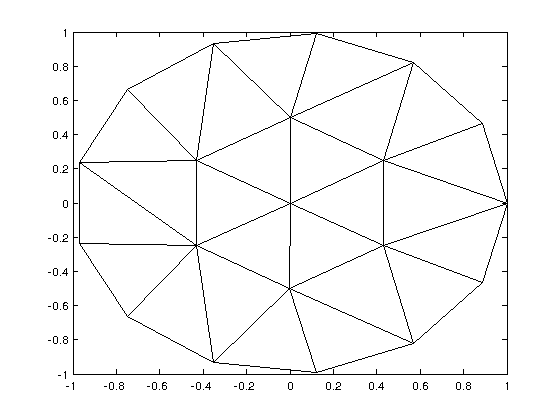
\includegraphics[width=\linewidth]{2d20.png}
  \caption{20 nodes}\label{fig:2d20}
\endminipage\hfill
\minipage{0.32\textwidth}
  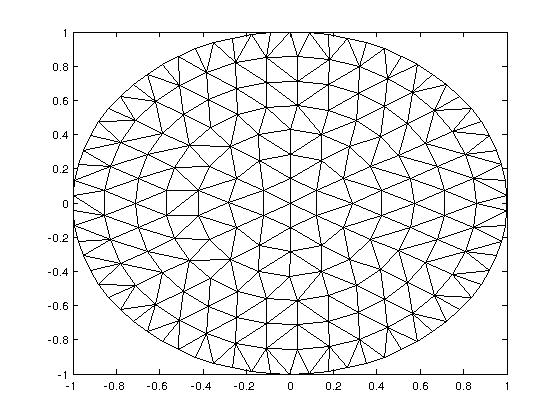
\includegraphics[width=\linewidth]{2d200.png}
  \caption{200 nodes}\label{fig:2d200}
\endminipage\hfill
\minipage{0.32\textwidth}
  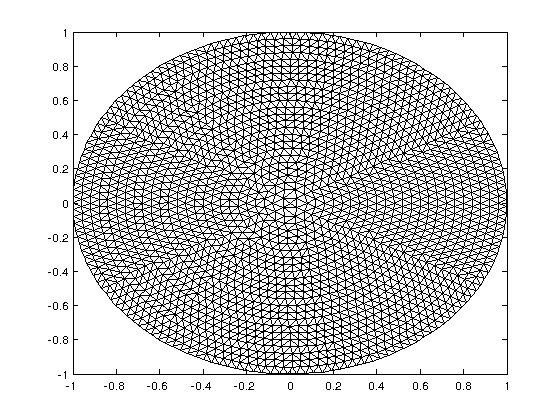
\includegraphics[width=\linewidth]{2d2000.png}
  \caption{2000 nodes}\label{fig:2d2000}
\endminipage
\end{figure}
Then build the stiffness matrix $A$ and loading vector $\mathbf{f}$.

\subsection{Stiffness matrix}
As shown earlier the elements of the stiffness matrix is given by

\[ A_{ij} = a(\phi_i,\phi_j)=\int_{\Omega} \nabla \phi_i \nabla \phi_j \mathrm{d}x\mathrm{d}y.\] 
Consider one element of the triangulation $K_k$ with corner points $\mathbf{p_\alpha}=(x_\alpha,y_\alpha)$, $\alpha=1,2,3$. Since the basis functions are linear they are uniquely determined by three coefficients, i.e

\[\phi_\alpha(x,y) = a_\alpha +b_\alpha x+c_\alpha y.\]

The Kronecker delta-property of the basis functions then gives that $(a_1, b_1,c_1)$ is governed by the equations $\phi_1(x_1,y_1)=1$, $\phi_1(x_2,y_2)=0$ and $\phi_1(x_3,y_3)=0$, or written in matrix form

\begin{equation}
\begin{bmatrix}
  1 & x_1 & y_1\\
  1 & x_2 & y_2\\
  1 & x_3 & y_3\\\end{bmatrix}
\begin{bmatrix} a_1 \\ b_1\\ c_1 \\ \end{bmatrix} =
\begin{bmatrix}
  1 \\ 0\\ 0 \\
\end{bmatrix}.
\label{eq:poisson2d:C-matrix}
\end{equation}

Similarly one can find $(a_2, b_2,c_2)$ and $(a_3, b_3,c_3)$. Note that $\nabla \phi_\alpha=(b_\alpha,c_\alpha)$, and hence the gradients are independent of $x$ and $y$ and can be moved outside the integral. The elements of the local stiffness matrix is thus given by

\[ A^K_{\alpha\beta} =\nabla \phi_\alpha \nabla \phi_\beta \int_{K} \mathrm{d}x\mathrm{d}y = \nabla \phi_\alpha \nabla \phi_\beta T_K.\]

This reduces the problem to solving (\ref{eq:poisson2d:C-matrix}) for the gradients and using equation (\ref{eq:jacobian2d}) from section 1.2 to find $T_K$.

To build the whole matrix A loop over each element and pick out the corner points. Then for each combination of basis functions (9 per element) add the scaled contribution to the full matrix.

TODO: SOMETHING ABOUT WHY THE A-matrix is singular.(Have not removed the nodes corresponding to the boundary conditions)
\subsection{Loading vector}
The elements of vector $\mathbf{f}$ is given by
\[ f_i = l(\phi_i) = \int_{\Omega}f\phi_i\mathrm{d}x\mathrm{d}y.\]

Remember that $\phi_i(\mathbf{p_j})=\delta_{ij}$ and that $\phi_i$ is linear. This means that $f\phi_i$ only has support (i.e. is different from zero) on triangles in which $\mathbf{p_i}$ is one of the corner nodes. It is therefore smart to find the contribution to $f_i$ from the triangles around $\mathbf{p_i}$. Consider some element $K$. Using the quadrature-rules from section 1.2 and local numbering $\alpha$ for the corners 

\[ l^{K}(\phi_\alpha) = \int_{K}f\phi_\alpha\mathrm{d}x\mathrm{d}y \approx T_K \sum\limits^{3}_{q=1} \rho_q f(\mathbf{x}_q)\zeta_\alpha(q) \qquad \alpha =1,2,3\]

where $\zeta_\alpha(q)$ is the $q$'th element of the quadrature rule and $\mathbf{x}_\alpha=\sum^3_{j=1}\zeta_\alpha(j)\mathbf{p}_j$. Do this for the three quadrature points $\mathbf{x_\alpha}$ to get the contribution to $\mathbf{f}$ from $K$ corresponding to the basis function at the corner nodes. Now iterate over the elements and add to the total vector $\mathbf{f}$ at appropriate indices.
\subsection{Boundary conditions}
To force the boundary condition in (\ref{eq:poisson2d}), $u$ has to be zero on the boundary. This can be done in the following way. Seperate the internal nodes and edge nodes into two arrays. Remove the rows and columns in $A$ and element in $\mathbf{f}$ corresponding to the nodes at the boundary. Solve the reduced linear system $A_\mathrm{int}\mathbf{u}_\mathrm{int}=\mathbf{f}_\mathrm{int}$, which is no longer singular. Construct $\mathbf{u}$ again from $\mathbf{u}_\mathrm{int}$ and letting the edge nodes be zero.  

\subsection{Verification}
TODO: Compare analytical and FE solution
\begin{figure}[!htb]
\minipage{0.5\textwidth}
  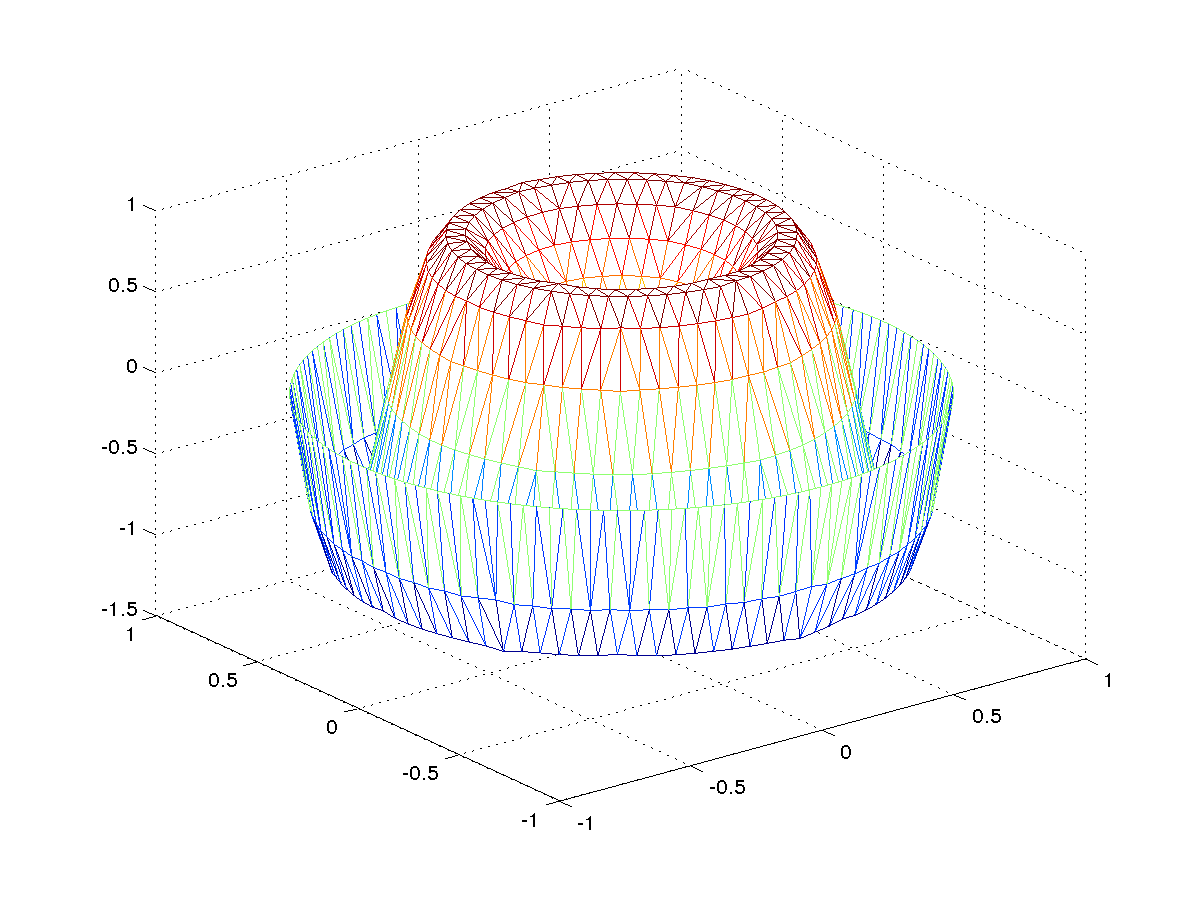
\includegraphics[width=\linewidth]{2h1000.png}
  \caption{Numerical solution of (\ref{eq:poisson2d}) with 1000 nodes}\label{fig:2h1000}
\endminipage\hfill
\minipage{0.5\textwidth}
  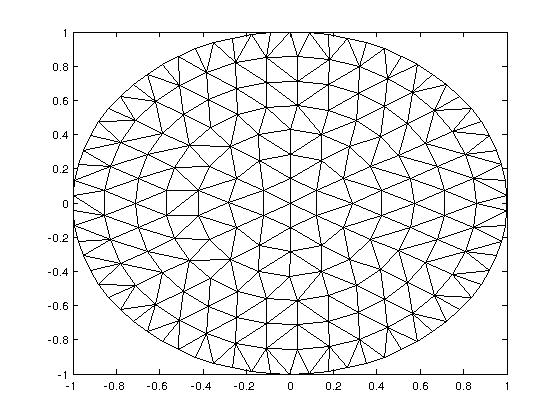
\includegraphics[width=\linewidth]{2d200.png}
  \caption{ERROR PLOT?}\label{fig:2d200}
\endminipage\hfill
\end{figure}


\section{Neumann boundary conditions}
Consider now the Poisson problem in 2D with Neumann boundary condition
\begin{equation}
\begin{aligned}
\nabla^2u(x,y) 	&= -f(x,y) \\
\left. u(x,y)\right|_{\partial\Omega_D} 	&= 0, \\
\left. \frac{\partial u(x,y)}{\partial n}\right|_{\partial\Omega_N} &= g(x,y).
\end{aligned}
\label{eq:poisson2d:Neu:problem}
\end{equation}
The source term $f$ and exact solution $u$ is still as in (\ref{eq:poisson2d}) and (\ref{eq:poisson2danal}), and $g$ is given by

\begin{equation}
g(r,\theta) =4\pi r\cos(2\pi r^2).
\label{eq:poisson2d:Neu:condition}
\end{equation}
The boundary domains are given by $\partial\Omega_D = \{x^2+y^2=1,y<0\}$ and $\partial\Omega_N = \{x^2+y^2=1,y>0\}$.

\subsection{Boundary condition}
Equation (\ref{eq:poisson2danal}) is a solution to (\ref{eq:poisson2d:Neu:problem}) also on the Neumann boundary since from \eqref{eq:poisson2d:Neu:condition}
\[\left. \frac{\partial u(x,y)}{\partial n}\right|_{\partial\Omega_N} = \frac{\partial}{\partial r} \sin(2\pi r^2) = 4\pi r\cos(2\pi r^2) = g(x,y).\]
\subsection{Variational formulation}
With the introduction of the new boundary condition the weak formulation changes. As before take a test function $v\in V$ and integrate over the domain. Using Green's theorem we get

\[\int_{\Omega}  (\nabla^2u)v = \int_{\partial\Omega_D} (\partial_n u) v + \int_{\partial\Omega_N} (\partial_n u) v-\int_{\Omega} \nabla u \cdot \nabla v = -\int_{\Omega} f v,\]
or 
\[\int_{\Omega} \nabla u \cdot \nabla v = \int_{\Omega} f v +  \int_{\partial\Omega_N} \! g v\]
if $v\in V= H^1_{\partial\Omega_D}(\Omega) = \{u\in H^1(\Omega) : u=0 \; \mathrm{on} \;  \partial\Omega_D\}$.

Hence it is similar to solving $A\mathbf{u}=\mathbf{f}$ for the Dirichlet case, only that $l(\cdot)$ changes to

\begin{equation}
l(v)=\int_{\Omega} f v  +  \int_{\partial\Omega_N} \! g v
\label{eq:poisson2d:l}
\end{equation}
\subsection{Gauss quadrature revisit}
Now to construct the $\mathbf{f}$-vector we need to evaluate line integrals on the boundary. The method in section 1.1 is changed slightly to work for points given on a plane. Consider a line segment $\Omega$ between points $p_1$ and $p_2$ on the (x,y)-plane. If $\hat{\Omega}=[-1,1]$ we get

\[ \mathbf{x}=\frac{1}{2} \left((\mathbf{p_2}-\mathbf{p_1}) \zeta +(\mathbf{p_2}+\mathbf{p_1})\right).\]

And 
\[ \int_{\Omega} \! g(x,y) \, \mathrm{d}x\mathrm{d}y \approx \frac{L}{2}\sum_{q=1}^{N_q} \rho_{q}g(\mathbf{x}(\zeta_q))
\]
where $L$ is the length of the line segment between $p_1$ and $p_2$.
\subsection{Implementation}
Now everything is set to solve the 2D Poisson problem with mixed boundary conditions given by \eqref{eq:poisson2d:Neu:problem}.
The stiffness matrix and loading vector is constructed as before, but now we need to keep track of which part of the boundary that should have Neumann and Dirichlet conditions. To do so we iterate over the edge nodes and split it into two vectors according to if it is above or below the $x$-axis.

Consider now one of the line segments on the Neumann boundary. Call this $L$ and let it be determined by its two end points $p_i$ and $p_j$. Each such segment has two basis functions associated with it, $\phi_{\alpha}(x,y)=a_{\alpha}x+b_{\alpha}y$. Now we need $\phi_{i}(p_i)=1$, $\phi_{i}(p_j)=0$, $\phi_{j}(p_j)=1$ and $\phi_{j}(p_i)=0$ or in matrix from for the first case

\[\begin{bmatrix}
  x_i & y_i\\
  x_j & y_j\\
 \end{bmatrix}
\begin{bmatrix} a_i \\ b_i\\ \end{bmatrix} =
\begin{bmatrix}
  1 \\ 0\\ 
\end{bmatrix}.\]

Solving this we can define $h_i(\mathbf{x})=g(\mathbf{x})\phi_i(\mathbf{x})$ and use from section 3.3 that 
\[
l^L(\phi_i)=\int_{L} \! g \phi_i = \int_{L} \! h(\mathbf{x}) \approx \frac{L}{2}\sum_{q=1}^{N_q} \rho_{q}h(\mathbf{x}(\zeta_q)).\]

Now iterate over all the Neumann edges and add the contribution to $\mathbf{f}$.

The next step is to remove the Dirichlet nodes, solve the system and add the nodes back into the solution vector $\mathbf{u}$.  Since our test problem has a Neumann boundary $g(x,y)$ that corresponds to the analytic solution we expect no difference in this implementation than from the solution of \eqref{eq:poisson2d} shown in figure \ref{fig:2h1000}. The result of the implementation is shown below in figure \ref{fig:3d5000}.

\begin{figure}[!htb]
  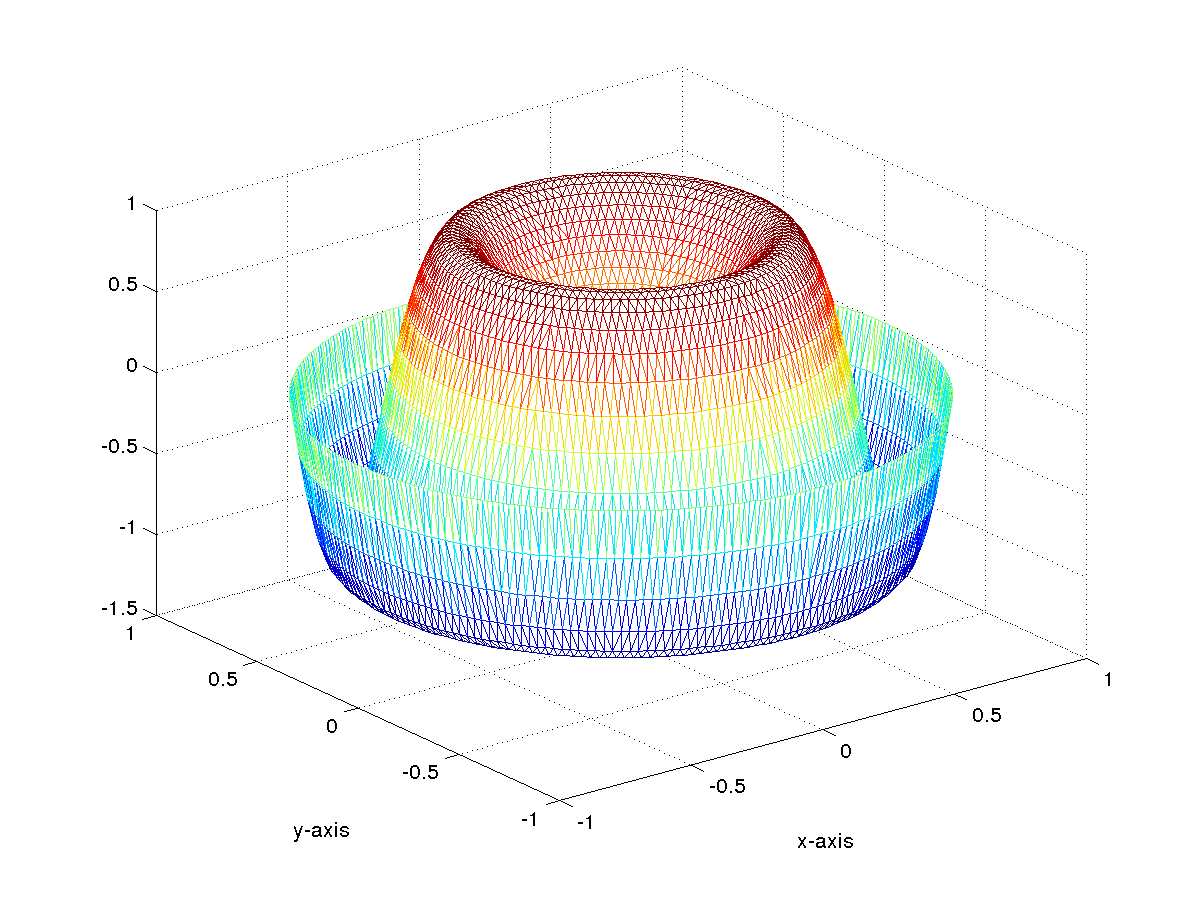
\includegraphics[width=\linewidth]{3d5000.png}
  \caption{Numerical solution of (\ref{eq:poisson2d:Neu:problem}) with 5000 nodes}\label{fig:3d5000}
\end{figure}

TODO: Compare solutions. How does your solution in the interior compare to the one you got in task 2? How does your solution at the boundary compare?

\section{Problems in 3 dimensions}
\subsection{The Poisson problem in 3D}
The next natural step is to go into three dimensions. We are then  solving
\begin{equation}
\begin{aligned}
\nabla^2 u 	&= -f \\
\left. u\right|_{\partial\Omega} 	&= 0, \\
\end{aligned}
\label{eq:poisson3d}
\end{equation}
for $u(x,y,z)$. We will use tetrahedral elements, solve it on the ball generated by \texttt{getSphere} and with

\[f(r,\phi,\theta) = -12\pi\cos(2\pi r^2) + 16\pi^2r^2\sin(2\pi r^2).\]

The modifications from the 2D case are minor. Take for instance system \eqref{eq:poisson2d:C-matrix} which now becomes

\[\begin{bmatrix}
  1 & x_1 & y_1 & z_1\\
  1 & x_2 & y_2 & z_2\\
  1 & x_3 & y_3 & z_3\\
  1 & x_4 & y_4 & z_4\\ \end{bmatrix}
\begin{bmatrix} a_1 \\ b_1\\ c_1 \\ d_1 \\ \end{bmatrix} =
\begin{bmatrix}
  1 \\ 0\\ 0 \\ 0 \\
\end{bmatrix},\]

and the loading uses 3D instead of 2D quadrature rules.
 
\subsection{Volume visualization}
In 3D it is not as easy to visualize the results, and we therefore consider two different approaches to show the values inside the ball. The first one is using isosurfaces in \textsc{Matlab}. This is a way to plot solutions corresponding to a constant $u$-value. The alternative is to use a dedicated visualizing program. We choose to use the open source alternative ParaView. The resulting plots are shown i figure \ref{fig:4b500} and \ref{fig:4b}.

\begin{figure}[!htb]
\minipage{0.45\textwidth}
  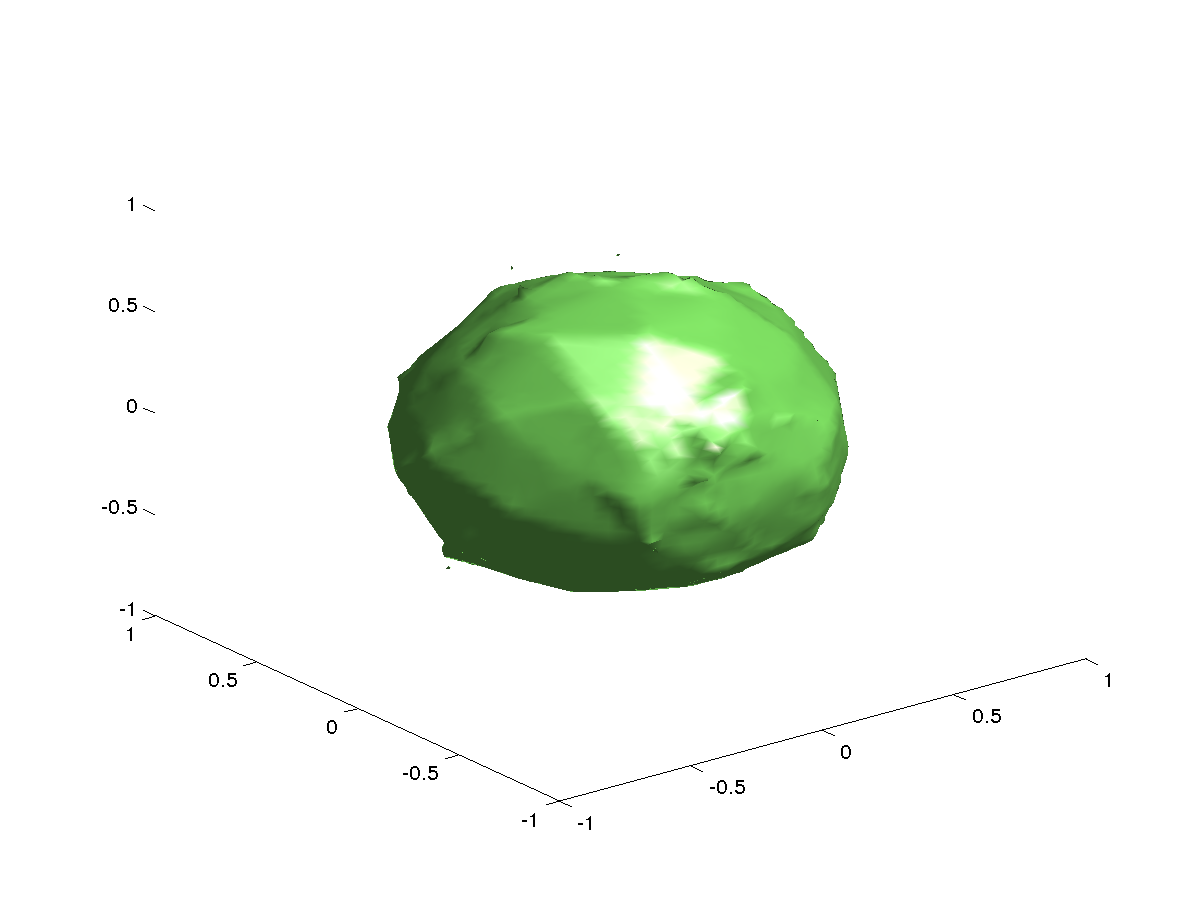
\includegraphics[width=\linewidth]{4b500.png}
  \caption{Numerical solution of (\ref{eq:poisson3d}) with 500 nodes using \textsc{Matlab}'s isosurfaces}\label{fig:4b500}
\endminipage\hfill
\minipage{0.45\textwidth}
  \includegraphics[width=\linewidth]{4b.png}
  \caption{Visualization of the solution using ParaView}\label{fig:4b}
\endminipage\hfill
\end{figure}

\subsection{Neumann boundary condition}
Finally we added the same Neumann condition as in the 2D case, but now for the top half of the ball ($z>0$). Again we need to split the boundary into the nodes with Neumann and Dirichlet conditions. Then we can use the idea from 3.4 adding a component to the spatial coordinates and hence doing a plane integral instead of a line integral for the boundary.

\end{document}